%**************************************************************************************
% License:
% CC BY-NC-SA 4.0 (http://creativecommons.org/licenses/by-nc-sa/4.0/)
%**************************************************************************************

\documentclass[notes]{beamer}

\mode<presentation> {

\usetheme{Madrid}

% Burnt orange
\definecolor{burntorange}{rgb}{0.8, 0.33, 0.0}
\colorlet{beamer@blendedblue}{burntorange}
% Pale yellow
\definecolor{paleyellow}{rgb}{1.0, 1.0, 0.953}
\setbeamercolor{background canvas}{bg=paleyellow}
% Secondary and tertiary palette
\setbeamercolor*{palette secondary}{use=structure,fg=white,bg=burntorange!80!black}
\setbeamercolor*{palette tertiary}{use=structure,fg=white,bg=burntorange!60!black}

% To remove the navigation symbols from the bottom of all slides uncomment this line
%\setbeamertemplate{navigation symbols}{}
}

% Custom note page template for longer notes
\setbeamertemplate{note page}{%
  \insertnote
}
\setbeameroption{show notes}

\usepackage{amsmath}
\DeclareMathOperator*{\argmin}{arg\,min}
\DeclareMathOperator*{\argmax}{arg\,max}
\usepackage{bm}
\usepackage{booktabs}
\usepackage{breqn}
\usepackage{cleveref}
\usepackage{graphicx}
\usepackage[labelsep=space,tableposition=top]{caption}
\renewcommand{\figurename}{Fig.}
\usepackage{caption,subcaption}
\usepackage{xcolor}
\usepackage{hyperref}
\usepackage{tikz}
\usetikzlibrary{positioning,calc}

%\AtBeginSection[]{
%	\begin{frame}{Outline}
%		\tableofcontents[
%		currentsection,
%		hideallsubsections
%		]
%	\end{frame}
%}

%----------------------------------------------------------------------------------------
%	TITLE PAGE
%----------------------------------------------------------------------------------------
\title[Neural ODEs]{Neural Ordinary Differential Equations}
\author{Krishna Kumar}
\institute[UT Austin]
{
University of Texas at Austin \\
\medskip
\textit{
  \url{krishnak@utexas.edu}}
}
\date{}

\begin{document}

\begin{frame}
\titlepage
\end{frame}

\begin{frame}
 \frametitle{Overview}
 \tableofcontents
\end{frame}

%----------------------------------------------------------------------------------------
% SLIDES
%----------------------------------------------------------------------------------------

\section{From ResNets to Continuous Dynamics}

%------------------------------------------------
\begin{frame}
\frametitle{Learning Objectives}

\begin{itemize}
    \item Understand the connection between ResNets and continuous dynamics
    \item Master the Neural ODE framework and adjoint method
    \item Implement ODENets for image classification
    \item Apply continuous normalizing flows for generative modeling
    \item Build latent ODE models for irregular time series
\end{itemize}

\vspace{1cm}
\centering
\href{https://colab.research.google.com/github/kks32-courses/sciml/blob/main/docs/08-neural-ode/neural-ode.ipynb}{\beamergotobutton{Open Notebook}}

\end{frame}

%------------------------------------------------
\begin{frame}
\frametitle{The ResNet Formula}

A residual network transforms hidden states layer by layer:

\begin{equation}
h_{t+1} = h_t + f(h_t, \theta_t)
\end{equation}

where $t \in \{0, 1, \ldots, T\}$ indexes the layers.

\vspace{0.5cm}

\begin{block}{The Key Question}
What happens as we add more layers ($T \to \infty$) and take smaller steps?
\end{block}


\end{frame}

%------------------------------------------------
\begin{frame}
\frametitle{The Euler Connection}

The ResNet update is the \textbf{Euler discretization} of an ODE:

\begin{equation}
\frac{dh(t)}{dt} = f(h(t), t, \theta)
\end{equation}

\vspace{0.5cm}

\begin{alertblock}{Key Insight}
A ResNet with infinitely many infinitesimal layers $\equiv$ solving an ODE
\end{alertblock}

\vspace{0.5cm}

Instead of specifying discrete layers, we parameterize the \textbf{derivative} of the hidden state using a neural network.


\end{frame}


%------------------------------------------------
\begin{frame}
	\frametitle{ResNet vs ODE}
	
	\begin{center}
		\includegraphics[width=0.7\textwidth]{figs/neuralode.png}
	\end{center}

\end{frame}

%------------------------------------------------
\begin{frame}
	\frametitle{ResNet vs ODE}

	\begin{center}
		\includegraphics[width=0.7\textwidth]{figs/resent-neuralode-arch.png}
	\end{center}

\end{frame}

%------------------------------------------------
\begin{frame}
\frametitle{Numerical Integration: From Discrete to Continuous}

\textbf{The Mathematician's View:}

The exact solution to $\frac{dx}{dt} = f(x, t, \theta)$ from time $t_k$ to $t_{k+1}$ is:

\begin{equation}
x_{k+1} = x_k + \int_{t=t_k}^{t=t_{k+1}} f(x(\tau), \tau, \theta) \, d\tau
\end{equation}

\vspace{0.3cm}

\textbf{The Problem:} We can't compute this integral analytically!

\vspace{0.3cm}

\textbf{The Solution:} Numerical integration schemes approximate this integral

\begin{itemize}
    \item \textbf{Euler (ResNet):} Simplest approximation, worst accuracy
    \item \textbf{Runge-Kutta:} Better approximations, higher accuracy
    \item \textbf{Adaptive methods:} Adjust step size automatically
\end{itemize}


\end{frame}

%------------------------------------------------
\begin{frame}
\frametitle{Integration Schemes: Euler (ResNet)}

\textbf{Euler Method (Forward Euler):}
\begin{equation}
x_{k+1} = x_k + \Delta t \cdot f(x_k, t_k, \theta)
\end{equation}

With $\Delta t = 1$: $x_{k+1} = x_k + f(x_k, \theta)$ \quad $\leftarrow$ ResNet!

\vspace{0.5cm}

\begin{center}
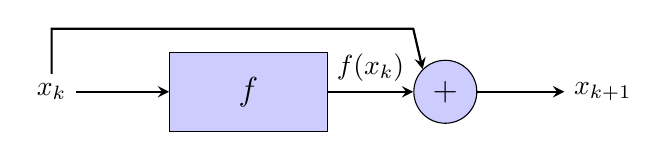
\begin{tikzpicture}[
    block/.style={rectangle, draw, fill=blue!20, minimum width=2cm, minimum height=1cm, font=\large},
    sum/.style={circle, draw, fill=blue!20, minimum size=0.8cm, font=\large},
    arrow/.style={->, >=stealth, thick}
]
    \node (input) at (0,0) {$x_k$};
    \node[block] (f) at (2.5,0) {$f$};
    \node[sum] (add) at (5,0) {$+$};
    \node (output) at (7,0) {$x_{k+1}$};

    \draw[arrow] (input) -- (f);
    \draw[arrow] (f) -- (add) node[midway, above] {$f(x_k)$};
    \draw[arrow] (add) -- (output);
    \draw[arrow] (input) |- ($(add.west) + (0,0.8)$) -- (add.north west);
\end{tikzpicture}
\end{center}

\vspace{0.3cm}

\textbf{Properties:}
\begin{itemize}
    \item One function evaluation per step
    \item First-order accurate: error $\mathcal{O}(\Delta t^2)$
    \item Simple but can be unstable
\end{itemize}


\end{frame}

%------------------------------------------------
\begin{frame}
\frametitle{Integration Schemes: Midpoint (2nd Order)}

\textbf{Midpoint Method (2nd order Runge-Kutta):}
\begin{align}
k_1 &= f(x_k, t_k, \theta) \\
x_{k+1} &= x_k + \Delta t \cdot f(x_k + \tfrac{\Delta t}{2} k_1, t_k + \tfrac{\Delta t}{2}, \theta)
\end{align}

\vspace{0.3cm}

\begin{center}
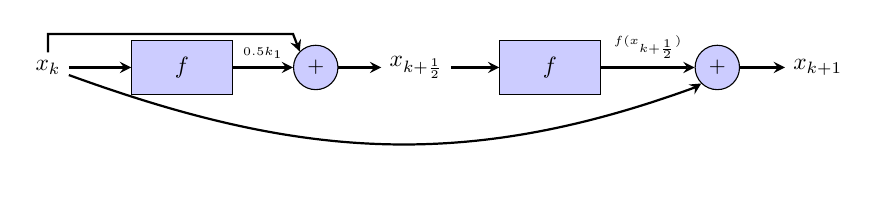
\begin{tikzpicture}[
    block/.style={rectangle, draw, fill=blue!20, minimum width=1.5cm, minimum height=0.8cm},
    sum/.style={circle, draw, fill=blue!20, minimum size=0.6cm, font=\small},
    arrow/.style={->, >=stealth, thick},
    scale=0.85, every node/.style={scale=0.85}
]
    \node (input) at (0,0) {$x_k$};
    \node[block] (f1) at (2,0) {$f$};
    \node[sum] (add1) at (4,0) {$+$};
    \node (mid) at (5.5,0) {$x_{k+\frac{1}{2}}$};
    \node[block] (f2) at (7.5,0) {$f$};
    \node[sum] (add2) at (10,0) {$+$};
    \node (output) at (11.5,0) {$x_{k+1}$};

    \draw[arrow] (input) -- (f1);
    \draw[arrow] (f1) -- (add1) node[midway, above, font=\tiny] {$0.5 k_1$};
    \draw[arrow] (add1) -- (mid);
    \draw[arrow] (mid) -- (f2);
    \draw[arrow] (f2) -- (add2) node[midway, above, font=\tiny] {$f(x_{k+\frac{1}{2}})$};
    \draw[arrow] (add2) -- (output);
    \draw[arrow] (input) |- ($(add1.west) + (0,0.5)$) -- (add1.north west);
    \draw[arrow] (input) to[out=-20, in=-160] ($(add2.west) + (0,-0.3)$) -- (add2.south west);
\end{tikzpicture}
\end{center}

\vspace{0.3cm}

\textbf{Properties:}
\begin{itemize}
    \item Two function evaluations per step
    \item Second-order accurate: error $\mathcal{O}(\Delta t^3)$
    \item Much more accurate than Euler for same $\Delta t$
\end{itemize}


\end{frame}

%------------------------------------------------
\begin{frame}
\frametitle{Integration Schemes: RK4 (4th Order)}

\textbf{Classical 4th Order Runge-Kutta (RK4):}
\begin{align}
k_1 &= f(x_k, t_k, \theta) \\
k_2 &= f(x_k + \tfrac{\Delta t}{2} k_1, t_k + \tfrac{\Delta t}{2}, \theta) \\
k_3 &= f(x_k + \tfrac{\Delta t}{2} k_2, t_k + \tfrac{\Delta t}{2}, \theta) \\
k_4 &= f(x_k + \Delta t \cdot k_3, t_k + \Delta t, \theta) \\
x_{k+1} &= x_k + \frac{\Delta t}{6}(k_1 + 2k_2 + 2k_3 + k_4)
\end{align}

\vspace{0.3cm}

\textbf{Properties:}
\begin{itemize}
    \item Four function evaluations per step
    \item Fourth-order accurate: error $\mathcal{O}(\Delta t^5)$
    \item Industry standard for non-stiff ODEs
    \item Much more stable than Euler/Midpoint
\end{itemize}


\end{frame}

%------------------------------------------------
\begin{frame}
\frametitle{ResNet vs Neural ODE}

\begin{columns}[c]

\column{.5\textwidth}
\textbf{Residual Network}
\begin{itemize}
    \item Discrete transformations
    \item Fixed number of layers $T$
    \item $x_{k+1} = x_k + f(x_k, \theta_k)$
    \item Memory: $\mathcal{O}(T)$
    \item Evenly spaced time steps
\end{itemize}

\column{.5\textwidth}
\textbf{Neural ODE}
\begin{itemize}
    \item Continuous dynamics
    \item Adaptive depth
    \item $\frac{dx}{dt} = f(x(t), t, \theta)$
    \item Memory: $\mathcal{O}(1)$
    \item Irregular time steps OK
\end{itemize}

\end{columns}

\vspace{0.5cm}


\end{frame}

\section{Neural ODE Architecture}

%------------------------------------------------
\begin{frame}
	\frametitle{Basic Neural ODE Components}
	
	\begin{block}{1. ODE Function $f(h, t, \theta)$}
		Neural network that computes the derivative $\frac{dh}{dt}$
	\end{block}
	
	\begin{block}{2. ODE Solver}
		Integrates $h(t)$ from $t_0$ to $t_1$:
		\begin{equation}
			h(t_1) = h(t_0) + \int_{t_0}^{t_1} f(h(t), t, \theta) dt
		\end{equation}
	\end{block}
	
	\begin{block}{3. Adjoint Method}
		Computes gradients $\frac{\partial L}{\partial \theta}$ efficiently
	\end{block}


\end{frame}

%------------------------------------------------
\begin{frame}
\frametitle{Memory Efficiency: The Adjoint Method}

\textbf{Standard Backpropagation:}
\begin{itemize}
    \item Store all intermediate layer activations
    \item Memory: $\mathcal{O}(L)$ where $L$ = number of layers
\end{itemize}

\vspace{0.5cm}

\textbf{Adjoint Method:}
\begin{itemize}
    \item Solve a second ODE backwards in time
    \item Recompute forward states during backward pass
    \item Memory: $\mathcal{O}(1)$ independent of depth
\end{itemize}

\vspace{0.3cm}

The adjoint state $\lambda(t) = \frac{\partial L}{\partial h(t)}$ evolves as:

\begin{equation}
\frac{d\lambda(t)}{dt} = -\lambda(t)^T \frac{\partial f(h(t), t, \theta)}{\partial h}
\end{equation}




\end{frame}

%------------------------------------------------
\begin{frame}
\frametitle{The Adjoint Method Visualized}

\begin{center}
\includegraphics[width=0.7\textwidth]{figs/adjoint.png}
\end{center}

\begin{itemize}
    \item \textbf{Forward}: Solve ODE from $t_0$ to $t_1$
    \item \textbf{Backward}: Solve augmented ODE from $t_1$ to $t_0$
    \item Automatically handled by \texttt{odeint\_adjoint}
\end{itemize}


\end{frame}

\section{Training Neural ODEs}

%------------------------------------------------
\begin{frame}
\frametitle{The Training Challenge}

\textbf{What we're doing:} Learning the vector field $f(x, t, \theta)$

\vspace{0.3cm}

\textbf{The Process:}
\begin{enumerate}
    \item Tweak parameters $\theta$ of the neural network
    \item Numerically integrate along the vector field
    \item Compare integrated trajectory to observed data
    \item Minimize loss between prediction and data
\end{enumerate}

\vspace{0.3cm}

\textbf{Key Challenge:} Hidden states between observations

Data is sampled at discrete times: $t_0, t_1, t_2, \ldots$

But the trajectory flows continuously: $x(\tau)$ for all $\tau \in [t_0, t_1]$

\vspace{0.3cm}

\begin{alertblock}{The Question}
How do we compute gradients through the ODE solver without storing all intermediate states?
\end{alertblock}


\end{frame}

\section{Detailed Adjoint Method}

%------------------------------------------------
\section{Adjoint Intuition}

\begin{frame}
\frametitle{Step 1: A Concrete Constrained Problem}

\textbf{Goal:} Minimize $f(x, y) = x^2 + y^2$ subject to $x + y = 1$

\begin{itemize}
    \item Geometrically: find the closest point on the line $x + y = 1$ to the origin
    \item Naive elimination: substitute $y = 1 - x$ and minimize $g(x) = x^2 + (1 - x)^2$
    \item Differentiate $g'(x) = 4x - 2$, set to zero: $x = 1/2$ and $y = 1/2$
    \item Works in tiny problems, but elimination explodes with many constraints/variables
\end{itemize}

\begin{block}{Observation}
We need a reusable way to enforce constraints without eliminating variables one-by-one.
\end{block}

\end{frame}

%------------------------------------------------
\begin{frame}
\frametitle{Step 2: Lagrange Multipliers Refresher}

Introduce a multiplier $\lambda$ and form
\[
\mathcal{L}(x, y, \lambda) = x^2 + y^2 + \lambda(x + y - 1).
\]

\vspace{0.3cm}

Stationarity $\nabla \mathcal{L} = 0$ gives
\[
2x + \lambda = 0,\qquad 2y + \lambda = 0,\qquad x + y - 1 = 0.
\]

\begin{itemize}
    \item $\partial \mathcal{L}/\partial x = 2x + \lambda = 0$ (gradient in $x$ direction)
    \item $\partial \mathcal{L}/\partial y = 2y + \lambda = 0$ (gradient in $y$ direction)
    \item $\partial \mathcal{L}/\partial \lambda = x + y - 1 = 0$ (enforces the constraint)
\end{itemize}

\begin{enumerate}
    \item From $2x + \lambda = 0$ and $2y + \lambda = 0$ we get $x = -\lambda/2$ and $y = -\lambda/2$.
    \item Substitute into the constraint: $x + y - 1 = -\lambda - 1 = 0$.
    \item Therefore $\lambda = -1$ and $x = y = 1/2$.
\end{enumerate}

\begin{block}{Takeaway}
$\lambda$ tells us how sensitive the optimum is to the constraint $x + y = 1$. Relaxing the constraint by $\varepsilon$ would change the optimum by roughly $-\lambda\,\varepsilon$.
\end{block}

\end{frame}

%------------------------------------------------
\begin{frame}
\frametitle{Step 3: Introduce Parameters and Sensitivities}

Consider a general design parameter $s$:
\[
\min_{x} \; f(x, s) \quad \text{s.t.} \quad c(x, s) = 0.
\]

\begin{itemize}
    \item We already know how to find $x^\star(s)$.
    \item New question: how does the optimal value change as we change $s$?
    \item We want the sensitivity $df/ds$ evaluated at the optimum.
\end{itemize}

\begin{block}{Motivating Example}
Heated rod: $-u''(x) = s(x)$ with $u(0)=u(1)=0$, and cost
$J = \int_0^1 (u - u_{\text{target}})^2 \, dx$.
\end{block}

\end{frame}

%------------------------------------------------
\begin{frame}
\frametitle{Heated Rod Example}

\textbf{State (constraint):}
\[
-\frac{d^2 u}{dx^2} = s(x), \qquad u(0) = u(1) = 0.
\]

\textbf{Objective:}
\[
J(s) = \int_0^1 \big(u(x; s) - u_{\text{target}}(x)\big)^2 \, dx.
\]

\begin{itemize}
    \item $s(x)$ controls heater strength along the rod.
    \item We seek $dJ/ds(x)$: ``If I add heat here, how does the mismatch change?''
\end{itemize}

\end{frame}

%------------------------------------------------
\begin{frame}
\frametitle{Naive Sensitivity Strategies}

\begin{block}{Finite Differences}
Solve the PDE twice:
$u(s)$ and $u(s+\varepsilon)$, then
$dJ/ds \approx \frac{J(s+\varepsilon) - J(s)}{\varepsilon}$.
\begin{itemize}
    \item Requires one extra PDE solve per component of $s$.
    \item Prohibitively expensive when $s$ has many components.
\end{itemize}
\end{block}

\begin{block}{Forward Sensitivity}
Differentiate the constraint:
\[
\frac{\partial c}{\partial u}\frac{du}{ds} + \frac{\partial c}{\partial s} = 0.
\]
Solve for $du/ds$, then plug into
$dJ/ds = \frac{\partial J}{\partial u}\frac{du}{ds} + \frac{\partial J}{\partial s}$.
\begin{itemize}
    \item Still one large linear system \textbf{per component} of $s$.
\end{itemize}
\end{block}

\end{frame}

%------------------------------------------------
\begin{frame}
\frametitle{Adjoint Method in Three Lines}

\textbf{First attempt (forward sensitivity):}
\begin{align*}
c(u, s) &= 0 \quad \Rightarrow \quad \frac{\partial c}{\partial u}\frac{du}{ds} + \frac{\partial c}{\partial s} = 0,\\
\frac{du}{ds} &= -\left(\frac{\partial c}{\partial u}\right)^{-1}\frac{\partial c}{\partial s}, \\
\frac{dJ}{ds} &= \frac{\partial J}{\partial u}\frac{du}{ds} + \frac{\partial J}{\partial s}.
\end{align*}
\textbf{Issue:} Need to solve this linear system \emph{once per component} of $s$.

\vspace{0.25cm}
\end{frame}

%------------------------------------------------
\begin{frame}
\frametitle{Adjoint Method in Three Lines}


\textbf{Adjoint trick (one solve total):}
\begin{enumerate}
    \item Form $\mathcal{L}(u, s, \lambda) = J(u, s) + \lambda^\top c(u, s)$.
    \item Set $\partial \mathcal{L}/\partial u = 0$:
    \[
    \frac{\partial J}{\partial u} + \lambda^\top \frac{\partial c}{\partial u} = 0
    \quad \Rightarrow \quad
    \left(\frac{\partial c}{\partial u}\right)^\top \lambda = -\frac{\partial J}{\partial u}.
    \]
    Solve this once for $\lambda$; it depends on $(u, s)$ but not on the dimension of $s$.
    \item Stationarity in $s$ gives the gradient:
    \[
    \frac{dJ}{ds} = \frac{\partial J}{\partial s} + \lambda^\top \frac{\partial c}{\partial s}.
    \]
\end{enumerate}

\begin{block}{Result}
Solve \emph{one} adjoint system for $\lambda$ and reuse it to obtain all components of $dJ/ds$.
\end{block}

\end{frame}

%------------------------------------------------
\begin{frame}
\frametitle{Adjoint for the Heated Rod}

\begin{itemize}
    \item Constraint: $-\frac{d^2 u}{dx^2} = s(x)$.
    \item Objective: $J = \int (u - u_{\text{target}})^2 dx$.
\end{itemize}

\textbf{Adjoint PDE} (stationarity w.r.t. $u$):
\[
-\frac{d^2 \lambda}{dx^2} = -2\big(u - u_{\text{target}}\big),
\qquad \lambda(0) = \lambda(1) = 0.
\]

\textbf{Gradient (stationarity in $s$)}:
\[
\frac{dJ}{ds}(x) = -\lambda(x)
\]
(we can flip the sign convention if we prefer to work with $+\lambda$).


\begin{block}{Interpretation}
$\lambda(x)$ tells us how helpful a unit of heat at $x$ would be in reducing the cost.
\end{block}

\end{frame}

%------------------------------------------------
\begin{frame}
\frametitle{Deriving the Heated-Rod Adjoint (1/2)}

\textbf{Constraint (state equation):}
\[
c(u, s) = -\frac{d^2 u}{dx^2} - s(x) = 0.
\]

\textbf{Objective:}
\[
J(u) = \int_0^1 (u - u_{\text{target}})^2 \, dx.
\]

Form the Lagrangian
\[
\mathcal{L}(u, s, \lambda) = J(u) + \int_0^1 \lambda(x)\,c(u, s)\,dx.
\]

Stationarity with respect to $u$:
\[
\frac{\partial \mathcal{L}}{\partial u} = 2(u - u_{\text{target}}) - \frac{d^2 \lambda}{dx^2} = 0.
\]

\textbf{Resulting adjoint PDE:}
\[
-\frac{d^2 \lambda}{dx^2} = -2(u - u_{\text{target}}), \quad \lambda(0)=\lambda(1)=0.
\]

\end{frame}

%------------------------------------------------
\begin{frame}
\frametitle{Deriving the Heated-Rod Adjoint (2/2)}

Stationarity with respect to $s$ gives
\[
\frac{dJ}{ds}(x) = \frac{\partial J}{\partial s} + \lambda(x)\frac{\partial c}{\partial s} = -\lambda(x).
\]
Throughout these slides we adopt the sign convention where the reported gradient is $-\lambda(x)$ so that increasing $s$ follows the negative adjoint direction.

\begin{block}{Summary}
\begin{enumerate}
    \item Solve the forward problem $-u'' = s$.
    \item Solve the adjoint problem $-\lambda'' = -2(u - u_{\text{target}})$.
    \item Use $\frac{dJ}{ds}(x) = \lambda(x)$ to update heater strengths.
\end{enumerate}
\end{block}

\end{frame}

%------------------------------------------------
\begin{frame}
\frametitle{From Adjoint to Backpropagation}

\begin{itemize}
    \item Classical backpropagation = adjoint method for discrete layers.
    \item \textbf{Forward pass:} compute activations (state trajectory).
    \item \textbf{Backward pass:} propagate adjoint sensitivities (gradients) layer by layer.
\end{itemize}


\begin{block}{Key Analogy}
Weights $w_i$ play the role of $s_i$.
Layer activations are the state $u$.
The backward pass solves the discrete adjoint system.
\end{block}

\end{frame}

%------------------------------------------------
\begin{frame}
\frametitle{Neural ODE Adjoint in Practice}

\textbf{Forward dynamics:}
\[
\frac{dz}{dt} = f_\theta(z, t), \qquad z(t_0) = z_0.
\]

\textbf{Adjoint dynamics:}
\[
\frac{d\lambda}{dt} = -\lambda^\top \frac{\partial f_\theta}{\partial z}, \qquad
\lambda(t_1) = \frac{\partial \mathcal{L}}{\partial z(t_1)}.
\]

\textbf{Parameter gradient:}
\[
\frac{\partial \mathcal{L}}{\partial \theta} = -\int_{t_0}^{t_1} \lambda^\top
\frac{\partial f_\theta}{\partial \theta}\, dt.
\]


\begin{block}{Practical Pipeline}
One forward ODE solve for $z(t)$ + one backward adjoint ODE solve for $\lambda(t)$ = gradients for \emph{all} parameters with $\mathcal{O}(1)$ memory.
\end{block}

\end{frame}

%------------------------------------------------
\begin{frame}[fragile]
\frametitle{Algorithm 1: Adjoint Sensitivity Method}

\textbf{Input:} Dynamics $f$, loss $L$, initial state $h(t_0)$, times $t_0 < t_1$

\vspace{0.3cm}

\textbf{Forward Pass:}
\begin{enumerate}
    \item Solve ODE: $h(t_1) = h(t_0) + \int_{t_0}^{t_1} f(h(t), t, \theta) \, dt$
    \item Compute loss: $L = L(h(t_1))$
\end{enumerate}

\vspace{0.3cm}

\textbf{Backward Pass:} Define augmented state $s(t) = [\lambda(t), \frac{\partial L}{\partial \theta}(t), \frac{\partial L}{\partial t_0}(t)]$

Initialize: $\lambda(t_1) = \frac{\partial L}{\partial h(t_1)}$, others zero

\vspace{0.2cm}

Solve augmented ODE backward from $t_1$ to $t_0$:
\begin{align*}
\frac{d\lambda(t)}{dt} &= -\lambda(t)^T \frac{\partial f(h(t), t, \theta)}{\partial h} \\
\frac{d}{dt}\frac{\partial L}{\partial \theta} &= -\lambda(t)^T \frac{\partial f(h(t), t, \theta)}{\partial \theta} \\
\frac{d}{dt}\frac{\partial L}{\partial t_0} &= -\lambda(t)^T f(h(t), t, \theta)
\end{align*}



\end{frame}

%------------------------------------------------
\begin{frame}
\frametitle{The Flow Map: Integral Form of Neural ODE}

\textbf{Definition:} The flow map $\Phi$ integrates the ODE from $t_0$ to $t_1$:

\begin{equation}
z(t_1) = \Phi(z(t_0), t_0, t_1, \theta) = z(t_0) + \int_{t_0}^{t_1} f(z(\tau), \tau, \theta) \, d\tau
\end{equation}

\vspace{0.3cm}

\textbf{Key Properties:}
\begin{itemize}
    \item $\Phi$ is the exact solution operator of the ODE
    \item Depends on initial condition $z(t_0)$, time interval, and parameters $\theta$
    \item Computed numerically via ODE solver (Euler, RK4, etc.)
    \item Differentiable with respect to all inputs!
\end{itemize}

\vspace{0.3cm}

\textbf{The Loss Function:}
\begin{equation}
L = L(z(t_1)) = L(\Phi(z(t_0), t_0, t_1, \theta))
\end{equation}

\textbf{The Training Problem:} Compute $\frac{dL}{d\theta}$ efficiently


\end{frame}

%------------------------------------------------
\begin{frame}
\frametitle{The Gradient Challenge}

\textbf{What we want:} $\frac{dL}{d\theta}$ where $L = L(\Phi(z(t_0), t_0, t_1, \theta))$

\vspace{0.3cm}

\textbf{Chain rule attempt:}
\begin{equation}
\frac{dL}{d\theta} = \frac{\partial L}{\partial z(t_1)} \frac{\partial z(t_1)}{\partial \theta}
\end{equation}

\vspace{0.3cm}

\textbf{The Problem:} Computing $\frac{\partial z(t_1)}{\partial \theta}$ requires tracking how parameters affect the entire trajectory!

\begin{equation}
\frac{\partial z(t_1)}{\partial \theta} = \frac{\partial}{\partial \theta}\left[z(t_0) + \int_{t_0}^{t_1} f(z(\tau), \tau, \theta) d\tau\right]
\end{equation}

This requires $\frac{\partial z(\tau)}{\partial \theta}$ for all $\tau \in [t_0, t_1]$ (the hidden states!)

\vspace{0.3cm}

\begin{alertblock}{The Core Issue}
Can't pull $\frac{\partial}{\partial \theta}$ inside the integral because $z(\tau)$ itself depends on $\theta$!
\end{alertblock}


\end{frame}

%------------------------------------------------
\begin{frame}
\frametitle{Lagrange Multipliers: The Setup}

\textbf{Constrained Optimization:} Minimize $L(z(t_1))$ subject to $\frac{dz}{dt} = f(z, t, \theta)$

\vspace{0.3cm}

\textbf{Key Idea:} Turn constraint into penalty using Lagrange multiplier $\lambda(t)$

\begin{equation}
\mathcal{L} = L(z(t_1)) - \int_{t_0}^{t_1} \lambda(t)^T \left[\frac{dz}{dt} - f(z(t), t, \theta)\right] dt
\end{equation}

\vspace{0.3cm}

\textbf{Why This Helps:}
\begin{itemize}
    \item When constraint is satisfied: $\frac{dz}{dt} = f$ so integral = 0
    \item Thus: $\mathcal{L} = L(z(t_1))$ (Lagrangian equals original loss)
    \item So: $\frac{d\mathcal{L}}{d\theta} = \frac{dL}{d\theta}$ (what we want!)
    \item But: We get to choose $\lambda(t)$ strategically!
\end{itemize}

\vspace{0.3cm}

\begin{block}{The Strategy}
Choose $\lambda(t)$ to eliminate the problematic $\frac{\partial z(\tau)}{\partial \theta}$ terms
\end{block}


\end{frame}

%------------------------------------------------
\begin{frame}
\frametitle{Deriving the Adjoint Equation (Step 1)}

\textbf{Expand the Lagrangian:}
\begin{equation}
\mathcal{L} = L(z(t_1)) - \int_{t_0}^{t_1} \lambda(t)^T \frac{dz}{dt} dt + \int_{t_0}^{t_1} \lambda(t)^T f(z(t), t, \theta) dt
\end{equation}

\vspace{0.3cm}

\textbf{Integration by Parts on the middle term:}
\begin{equation}
\int_{t_0}^{t_1} \lambda(t)^T \frac{dz}{dt} dt = \lambda(t_1)^T z(t_1) - \lambda(t_0)^T z(t_0) - \int_{t_0}^{t_1} \frac{d\lambda}{dt}^T z(t) dt
\end{equation}

\vspace{0.3cm}

\textbf{Substitute back:}
\begin{align}
\mathcal{L} = L(z(t_1)) &- \lambda(t_1)^T z(t_1) + \lambda(t_0)^T z(t_0) \\
&+ \int_{t_0}^{t_1} \left[\frac{d\lambda}{dt}^T z(t) + \lambda(t)^T f(z(t), t, \theta)\right] dt
\end{align}


\end{frame}

%------------------------------------------------
\begin{frame}
\frametitle{Deriving the Adjoint Equation (Step 2)}

\textbf{Take derivative with respect to $\theta$:}
\begin{align}
\frac{d\mathcal{L}}{d\theta} = &\frac{\partial L}{\partial z(t_1)} \frac{\partial z(t_1)}{\partial \theta} - \lambda(t_1)^T \frac{\partial z(t_1)}{\partial \theta} + \lambda(t_0)^T \frac{\partial z(t_0)}{\partial \theta} \\
&+ \int_{t_0}^{t_1} \left[\frac{d\lambda}{dt}^T \frac{\partial z}{\partial \theta} + \lambda(t)^T \left(\frac{\partial f}{\partial z} \frac{\partial z}{\partial \theta} + \frac{\partial f}{\partial \theta}\right)\right] dt
\end{align}

\vspace{0.3cm}

\textbf{Group terms with $\frac{\partial z}{\partial \theta}$:}
\begin{align}
\frac{d\mathcal{L}}{d\theta} = &\left(\frac{\partial L}{\partial z(t_1)} - \lambda(t_1)^T\right) \frac{\partial z(t_1)}{\partial \theta} \\
&+ \int_{t_0}^{t_1} \left[\left(\frac{d\lambda}{dt}^T + \lambda(t)^T \frac{\partial f}{\partial z}\right) \frac{\partial z}{\partial \theta}\right] dt \\
&+ \int_{t_0}^{t_1} \lambda(t)^T \frac{\partial f}{\partial \theta} dt
\end{align}

Note: $z(t_0)$ is fixed, so $\frac{\partial z(t_0)}{\partial \theta} = 0$


\end{frame}

%------------------------------------------------
\begin{frame}
\frametitle{The Adjoint Solution: Making Terms Vanish}

\textbf{Choose $\lambda(t)$ to eliminate all $\frac{\partial z}{\partial \theta}$ terms!}

\vspace{0.3cm}

\textbf{Boundary condition at $t_1$:}
\begin{equation}
\lambda(t_1)^T = \frac{\partial L}{\partial z(t_1)} \quad \Rightarrow \quad \text{Boundary term vanishes!}
\end{equation}

\vspace{0.3cm}

\textbf{Dynamics of $\lambda(t)$ (adjoint equation):}
\begin{equation}
\frac{d\lambda}{dt}^T = -\lambda(t)^T \frac{\partial f}{\partial z} \quad \Rightarrow \quad \text{Integral term vanishes!}
\end{equation}

\vspace{0.3cm}

\textbf{Final Gradient (what remains):}
\begin{equation}
\frac{dL}{d\theta} = \int_{t_0}^{t_1} \lambda(t)^T \frac{\partial f}{\partial \theta} dt = -\int_{t_1}^{t_0} \lambda(t)^T \frac{\partial f}{\partial \theta} dt
\end{equation}

\vspace{0.3cm}

\begin{alertblock}{Key Result}
$\lambda(t) =$ adjoint state, solve backward from $t_1$ to $t_0$, then compute gradient!
\end{alertblock}


\end{frame}

%------------------------------------------------
\begin{frame}
\frametitle{How Neural ODEs Automate This}

\textbf{The Traditional Way (Impossible):}
\begin{enumerate}
    \item Derive adjoint equations by hand for your specific $f$
    \item Compute Jacobians $\frac{\partial f}{\partial z}$ and $\frac{\partial f}{\partial \theta}$ analytically
    \item Implement custom backward pass
\end{enumerate}

\vspace{0.3cm}

\textbf{The Neural ODE Way (Automatic):}
\begin{enumerate}
    \item Define $f(z, t, \theta)$ as a neural network in PyTorch/JAX
    \item \textbf{Autodiff gives you $\frac{\partial f}{\partial z}$ and $\frac{\partial f}{\partial \theta}$ for FREE!}
    \item Solve adjoint ODE using same ODE solver, but backward
\end{enumerate}

\vspace{0.3cm}

\begin{block}{The Magic of Autodiff}
\textbf{Vector-Jacobian Products (VJPs):} \\
$\lambda(t)^T \frac{\partial f}{\partial z}$ and $\lambda(t)^T \frac{\partial f}{\partial \theta}$ \\
computed via reverse-mode autodiff without forming full Jacobian!
\end{block}

\vspace{0.3cm}

\textbf{Complexity:} VJP costs $\approx$ 2-3× forward pass (not O(d²) for Jacobian!)


\end{frame}

%------------------------------------------------
\begin{frame}
\frametitle{Adjoint Method: Why $\mathcal{O}(1)$ Memory?}

\textbf{Standard Backprop through ODE Solver:}
\begin{itemize}
    \item Store all intermediate states $h(t_i)$ for $i = 1, \ldots, N$
    \item $N$ depends on adaptive step size (could be 100s or 1000s)
    \item Memory: $\mathcal{O}(N)$ where $N$ = number of function evaluations
\end{itemize}

\vspace{0.5cm}

\textbf{Adjoint Method:}
\begin{itemize}
    \item Only store final state $h(t_1)$
    \item During backward pass, recompute $h(t)$ as needed
    \item Memory: $\mathcal{O}(1)$ -- just the current state!
\end{itemize}

\vspace{0.5cm}

\begin{alertblock}{Trade-off}
Memory $\mathcal{O}(1)$ but computation $\approx 2\times$ (one forward, one backward solve)
\end{alertblock}


\end{frame}


%------------------------------------------------
\begin{frame}
\frametitle{Hyperparameter Selection}

\begin{block}{ODE Solver Tolerance}
\begin{itemize}
    \item \texttt{rtol}, \texttt{atol}: Control accuracy
    \item Higher tolerance $\to$ faster but less accurate
    \item Typical: \texttt{rtol=1e-3}, \texttt{atol=1e-4}
\end{itemize}
\end{block}

\begin{block}{Solver Method}
\begin{itemize}
    \item \textbf{Adaptive}: 'dopri5', 'adams' (recommended)
    \item \textbf{Fixed-step}: 'euler', 'rk4' (for debugging)
\end{itemize}
\end{block}

\begin{block}{Integration Time}
\begin{itemize}
    \item Usually $T = 1.0$ (can be learned)
    \item Longer $T$ $\to$ more expressive but slower
\end{itemize}
\end{block}


\end{frame}

\section{Applications}

%------------------------------------------------
\begin{frame}
\frametitle{Latent ODEs for Irregular Time Series}

\textbf{Challenge:} Irregular, sparse observations with variable time gaps

\vspace{0.3cm}

\textbf{Approach:} Combine RNNs and ODEs
\begin{itemize}
    \item \textbf{Encoder (ODE-RNN):} Process observations backward in time
    \item \textbf{Latent ODE:} Smooth dynamics in continuous time
    \item \textbf{Decoder:} Generate predictions at any time
\end{itemize}

\vspace{0.3cm}

\textbf{Key Innovation:} Poisson process prior for observation times
\begin{equation}
p(t_1, \ldots, t_N | z_0) = \prod_{i=1}^N \lambda(t_i | z_0) \exp\left(-\int_0^T \lambda(t | z_0) dt\right)
\end{equation}

Models \emph{when} observations occur, not just their values.


\end{frame}

%------------------------------------------------
\begin{frame}
\frametitle{Latent ODE Architecture Details}

\begin{center}
\textbf{Three-Component System}
\end{center}

\begin{block}{1. ODE-RNN Encoder (Backward)}
Process observations $\{(t_i, x_i)\}_{i=1}^N$ in \emph{reverse} time order:
$$h_i = \text{ODESolve}(h_{i+1}, t_{i+1} \to t_i) \quad \text{then} \quad h_i \leftarrow \text{RNN}(h_i, x_i)$$
Output: Initial latent state $z_0 \sim q(z_0 | x_{1:N})$
\end{block}

\begin{block}{2. Latent ODE Dynamics}
Continuous evolution in latent space:
$$\frac{dz(t)}{dt} = f_\theta(z(t), t)$$
\end{block}

\begin{block}{3. Decoder}
Map latent states to observations: $p(x_i | z(t_i))$
\end{block}

\note[item]{
\textbf{Why Process Backward?} This is a key design choice! Processing observations backward in time naturally produces an initial condition $z_0$ that encodes the entire sequence. Think of it like reverse-engineering the initial state from the trajectory.

\textbf{The ODE-RNN Step:} At each observation time $t_i$ (going backward):
\begin{enumerate}
\item Evolve hidden state from $t_{i+1}$ to $t_i$ using an ODE: this accounts for the time gap
\item Update with RNN cell using observation $x_i$: this incorporates the data
\end{enumerate}

This is different from standard RNNs which assume fixed time steps. The ODE naturally handles variable gaps!

\textbf{Why This Architecture Works:}
\begin{itemize}
\item Encoder handles irregularity by explicitly modeling time via ODEs
\item Latent space has smooth, continuous dynamics (good inductive bias)
\item Can query $z(t)$ at any time, not just observation points
\item Decoder can make predictions at arbitrary future times
\end{itemize}
}


\end{frame}

%------------------------------------------------
\begin{frame}
\frametitle{Training Latent ODEs: The ELBO}

\textbf{Evidence Lower Bound (ELBO):} Variational inference objective

\vspace{0.3cm}

\begin{equation}
\mathcal{L}_{\text{ELBO}} = \underbrace{\mathbb{E}_{q(z_0|x)}[\sum_{i=1}^N \log p(x_i | z(t_i))]}_{\text{Reconstruction}} - \underbrace{D_{KL}(q(z_0|x) \| p(z_0))}_{\text{Regularization}}
\end{equation}

\vspace{0.3cm}

\textbf{Component 1: Reconstruction Loss}
\begin{itemize}
\item Measures how well the model predicts observations
\item $q(z_0|x)$: Encoder's posterior over initial state
\item $z(t_i)$: Latent state at time $t_i$ via ODE
\item Typically Gaussian: $\log p(x_i | z(t_i)) = \log \mathcal{N}(x_i | \mu(z(t_i)), \sigma^2)$
\end{itemize}

\textbf{Component 2: KL Divergence}
\begin{itemize}
\item Regularizes latent space to match prior $p(z_0) = \mathcal{N}(0, I)$
\item Prevents overfitting and ensures smooth latent space
\item Only computed at $t=0$, not entire trajectory!
\end{itemize}




\end{frame}

%------------------------------------------------
\begin{frame}
\frametitle{Latent ODE: Handling Observation Times}

\textbf{Innovation:} Model \emph{when} observations occur, not just their values

\vspace{0.3cm}

\textbf{Poisson Process Intensity:}
\begin{equation}
\lambda(t | z_0) = g_\psi(z(t))
\end{equation}

where $g_\psi$ is a neural network mapping latent states to observation rates.

\vspace{0.3cm}

\textbf{Joint Likelihood:}
\begin{equation}
p(\{x_i, t_i\}_{i=1}^N | z_0) = \underbrace{\prod_{i=1}^N p(x_i | z(t_i))}_{\text{observations}} \times \underbrace{\prod_{i=1}^N \lambda(t_i | z_0) \exp\left(-\int_0^T \lambda(t | z_0) dt\right)}_{\text{timing}}
\end{equation}

\vspace{0.3cm}

The integral $\int_0^T \lambda(t | z_0) dt$ is computed by solving an ODE!


\end{frame}

%------------------------------------------------
\begin{frame}
\frametitle{Function Encoders with Neural ODEs}

\textbf{Goal:} Transfer learned dynamics to new systems without gradient updates

\vspace{0.3cm}

\textbf{Approach:} Learn a basis of dynamics
\begin{enumerate}
    \item Learn $K$ basis ODEs: $\frac{dz_i}{dt} = f_i(z_i, t)$ for $i = 1, \ldots, K$
    \item For new system: encode demonstrations $\to$ coefficients $\alpha_i$
    \item Predict: $\frac{dz}{dt} = \sum_{i=1}^K \alpha_i f_i(z, t)$
\end{enumerate}

\vspace{0.3cm}

\textbf{Key Idea:} Treat dynamics as vectors in a Hilbert space

Any trajectory $x(z, t)$ can be represented as: $x \approx \sum_{i=1}^K \alpha_i \phi_i$

\vspace{0.3cm}

\begin{alertblock}{Zero-Shot Transfer}
Compute coefficients $\alpha_i$ from demonstrations without any gradient updates!
\end{alertblock}

\note[item]{
\textbf{The Big Picture:} This is a fundamentally different approach to transfer learning. Instead of fine-tuning a model for each new task, we learn a \emph{dictionary of dynamics} that can be combined to represent new systems.

\textbf{Analogy to Fourier Series:} Any periodic function can be written as $f(x) = \sum_k a_k \sin(kx) + b_k \cos(kx)$. The sine and cosine functions form a basis. Given any function $f$, we can compute coefficients $a_k, b_k$ via integrals (inner products). We're doing the same thing, but with dynamical systems instead of functions!

\textbf{Why Neural ODEs?} Each basis element $\phi_i$ is itself a Neural ODE with dynamics $f_i$. During training, we learn multiple Neural ODEs simultaneously (like learning both sines and cosines). The training objective encourages the basis to span a diverse space of dynamics.

\textbf{Training Phase:}
\begin{itemize}
\item Train on multiple dynamical systems (e.g., different robot configurations, different physical parameters)
\item Each system has multiple demonstration trajectories
\item Learn basis functions $\phi_1, \ldots, \phi_K$ that can represent all training systems as linear combinations
\end{itemize}

\textbf{Test Phase (Zero-Shot):}
\begin{itemize}
\item Given a NEW system (never seen during training)
\item Observe a few demonstration trajectories
\item Compute coefficients $\alpha_i$ to represent the new system
\item Make predictions using $\sum \alpha_i \phi_i$
\end{itemize}

The key is: computing coefficients is fast (no training), but they can represent complex dynamics!
}


\end{frame}

%------------------------------------------------
\begin{frame}
\frametitle{Function Encoder: Implementation Details}

\textbf{Computing Demonstration Velocity:} Given demonstration points $\{(t_j, z_j)\}$:

\begin{itemize}
    \item \textbf{Direct differentiation:} If demonstration is a continuous function, compute $\frac{dz}{dt}$ numerically
    \item \textbf{Finite differences:} For discrete observations: $v(t_j) \approx \frac{z_{j+1} - z_j}{t_{j+1} - t_j}$
\end{itemize}

\vspace{0.3cm}

\textbf{Inner Product Formula:}
\begin{equation}
\alpha_i = \mathbb{E}_{t \sim \mathcal{U}[0, T], z \sim z_i(t)}[\underbrace{v_{\text{demo}}(z, t)}_{\text{demo velocity}} \cdot \underbrace{f_i(z, t)}_{\text{basis velocity}}]
\end{equation}

\vspace{0.3cm}

\textbf{Key Properties:}
\begin{itemize}
    \item $\alpha_i > 0$: demonstration aligns with basis $i$
    \item $\alpha_i < 0$: demonstration opposes basis $i$
    \item $|\alpha_i|$ large: basis $i$ is important for this system
\end{itemize}


\end{frame}

%------------------------------------------------
\begin{frame}
\frametitle{Extensions}

\begin{block}{Augmented Neural ODEs}
Add extra dimensions to avoid topological constraints
\end{block}

\begin{block}{Second-order Neural ODEs}
Include acceleration: $\frac{d^2h}{dt^2} = f(h, \frac{dh}{dt}, t)$
\end{block}

\begin{block}{Stochastic Differential Equations (SDEs)}
Add noise for uncertainty: $dh = f(h, t)dt + g(h, t)dW$
\end{block}

\begin{block}{Hamiltonian Neural Networks}
Preserve energy and symplectic structure
\end{block}


\end{frame}

%------------------------------------------------
\begin{frame}
\frametitle{Practical Tip: Neural ODEs + Interpretable Models}

\textbf{Problem:} Neural ODEs are powerful but not interpretable

$f(x, t, \theta)$ is a black-box neural network -- can't extract equations!

\vspace{0.5cm}

\textbf{Solution:} Use Neural ODEs as a preprocessing step

\begin{enumerate}
    \item Train Neural ODE on irregular/noisy data
    \item Generate clean, regularly-spaced data from trained Neural ODE
    \item Pass regular data to interpretable method (SINDy, symbolic regression)
\end{enumerate}

\vspace{0.5cm}

\begin{block}{Best of Both Worlds}
Neural ODE: handles irregular data, noise robust, accurate

SINDy/Symbolic: gives interpretable equations like $\dot{x} = \mu x - x^3$
\end{block}


\end{frame}

%------------------------------------------------
\begin{frame}
\frametitle{Summary}

\begin{block}{Key Takeaways}
\begin{enumerate}
    \item Neural ODEs = continuous-depth neural networks
    \item ResNets are crude Euler integration; Neural ODEs use better solvers
    \item Adjoint method enables $\mathcal{O}(1)$ memory training via autodiff
    \item Works with irregular time series (unlike ResNets/RNNs)
    \item Can bake in physical structure (Hamiltonian, Lagrangian, symplectic)
    \item Applications: classification, time series, generative models, physics
\end{enumerate}
\end{block}

\vspace{0.3cm}

\begin{block}{The Big Idea}
Learn the \textbf{vector field} (continuous dynamics), not discrete transformations
\end{block}

\vspace{0.3cm}

\textbf{Key advantage:} Leverage 300+ years of ODE theory and numerical methods!

\end{frame}

%------------------------------------------------
\begin{frame}
\frametitle{References}

\begin{thebibliography}{99}

\bibitem{chen2018} Chen, R. T. Q., Rubanova, Y., Bettencourt, J., \& Duvenaud, D. (2018).
\newblock Neural Ordinary Differential Equations.
\newblock \textit{NeurIPS 2018} (Best Paper Award).

\bibitem{grathwohl2019} Grathwohl, W., Chen, R. T. Q., Bettencourt, J., Sutskever, I., \& Duvenaud, D. (2019).
\newblock FFJORD: Free-form Continuous Dynamics for Scalable Reversible Generative Models.
\newblock \textit{ICLR 2019}.

\bibitem{rubanova2019} Rubanova, Y., Chen, R. T. Q., \& Duvenaud, D. (2019).
\newblock Latent ODEs for Irregularly-Sampled Time Series.
\newblock \textit{NeurIPS 2019}.

\end{thebibliography}

\end{frame}


%----------------------------------------------------------------------------------------

\end{document}
